%\documentstyle[nips14submit_09,times,art10]{article} % For LaTeX 2.09
\documentclass{article} % For LaTeX2e
\usepackage{nips14submit_e,times}
\usepackage{hyperref}
\usepackage{url}
\usepackage{subcaption}
\usepackage{wrapfig}
\usepackage{amsmath}
\usepackage{framed}
\usepackage{color}
\definecolor{shadecolor}{gray}{0.8}

\usepackage{natbib}
\bibliographystyle{apalike}

\usepackage{tikz}
\usetikzlibrary{bayesnet}

\renewcommand\phi\varphi
\DeclareMathOperator*{\argmax}{arg\,max}

\title{Inducing Semantic Frames on a Very Large Corpus of Syntactic-Ngrams}

\author{
    Noble, Bill\\
    \texttt{winobes@gmail.com}
    \and
    Drumm, Eli T.\\
    \texttt{etd@dte.li}
    \and
    Verdegaal, Jacob\\
    \texttt{jacob.verdegaal@student.uva.nl}
}

% The \author macro works with any number of authors. There are two commands
% used to separate the names and addresses of multiple authors: \And and \AND.
%
% Using \And between authors leaves it to \LaTeX{} to determine where to break
% the lines. Using \AND forces a linebreak at that point. So, if \LaTeX{}
% puts 3 of 4 authors names on the first line, and the last on the second
% line, try using \AND instead of \And before the third author name.

\newcommand{\fix}{\marginpar{FIX}}
\newcommand{\new}{\marginpar{NEW}}

\nipsfinalcopy % Uncomment for camera-ready version

\begin{document}


\maketitle


\begin{abstract}
We explore two models for the unsupervised induction of semantic frames on a 
very large corpus of verb-subject-object triples. Our work is bade on previous 
research that has had success on smaller, more focused data sets. By encouraging 
verb sparsity with a Dirichlet prior, one can improve on the results of our 
baseline model. We give some analysis of the frames that the improved model 
discovers, and suggest areas for further development.
\end{abstract}

\section{Introduction}
The growing body of digital publications contains too much information for a single human being to process; it is even hard to keep up to date on a particular topic. It would be useful to be aided by technology that creates reliable summarizations. As a natural language processing task, summarization consists of two parts: first, extract the semantic content of a text, and then represent it in a condensed human readable output. The first part of such a technology, extracting semantic content, is what we deal with in this project. This step may also be useful on its own, for example, in automatic stock trading systems. Knowing what is published about publicly traded companies at the moment of publication can increase prophet margins for so-called high-frequency trading algorithms. Semantic representations have applications in other natural language processing as well. For example, interlingua approaches to machine translation try to match sentences in the source and target language to a common generic semantic representation \cite{boas2005}.

Semantic content of a sentence can be represented in a frame. The main verb phrase of the sentence is the head of the frame and can be interpreted as predicate, representing the core of the episode described by the sentence. The trick is to find out what the arguments of the predicate are. In linguistics, argument selection is called case grammar \citep{dowty1991} and arguments (or roles) have specific names as \textit{agent - patient}. In computational systems names are not important and can be assigned when frame induction is complete.

The problem of semantic content can be illustrated by this simple example: \textit{'Alice buys a bread from the baker'} describes the exact same situation as \textit{`The baker sells Alice a bread'}. Thus the semantic content of these sentences can be represented in one frame, where the head of the frame represents the core of the episode or situation and involvement is expressed by assigning roles to things or people. In general these roles can be anything like location, time, manner etc. The frame for the sentences above is depicted in table \ref{framex}.
\begin{wraptable}{r}{.3\textwidth}
  \centering
 % \begin{table}
\begin{tabular}{|l l|}
  \hline
  \textit{\small predicate:\normalsize}&Transaction\\
  \hline
  \hline
  \textit{\small role 1:\normalsize} &baker\\
  \textit{\small role 2:\normalsize} &Alice\\
  \textit{\small role 3:\normalsize} &bread\\
  \hline
\end{tabular}
%\end{table}
\caption{Simple frame}
\label{framex}
\end{wraptable}
As the example above shows, the roles are represented by different syntactic parts of speech in both sentences: the object and subject are switched. Furthermore, the verbs are different. Even given the knowledge of specific verbs that bear the same meaning with switched subject/indirect-object, we need to generate semantic representations on top of syntax in order to let machines (act as if they) understand language and process new text in a meaningful way. Hence, automatic semantic analysis and representation is required for further automatization.

The FrameNet project \citep{framenet} is an ongoing manual effort to define frames which could be mapped onto text to give a semantic representation. But with the increasing amount of digital information, not to mention the inherent tediousness of building such a resource one word at a time, the prospect of (partially or completely) automating semantic frame induction is enticing. An automatic system could provide more complete descriptions of frames in current document banks and could better adapt to new words and evolving meanings.

In this project we investigate whether probabilistic latent-variable models can cluster verbs based on their meaning, which is inferred from the arguments with which it occurs. These clusters then make up a broader, but hopefully distinct, meaning. The data we use contains triples of verb-subject-object (see section \ref{data}), so induced frames contain only two roles. The models (described in section \ref{models}) induce frames based on the assumption the meaning of a verb relative to meaning of other verbs can be induced from its context. Hence the broader meaning is latent. To evaluate our models we use two metrics, one of which uses framenet data to check whether the induced frames are similar to clusters of verbs in framenet, the other to check whether the resulting frames are coherent, i.e. whether the found clusters are not completely random. See section \ref{results} for more detail.

%\section{Related Work}
We based our work on two papers: \textit{`Inducing a semantically annotated lexicon via em-based clustering.'} by \citeauthor{rooth1999} and \textit{`Learning frames from text with an unsupervised latent variable model.'} by \citeauthor{oconnor2013}. In the first article clustering is realized by applying expectation maximization on a simple cooccurance model. This model produces frames in the form of two distributions, one for the predicate, a distribution over verbs, and one for the arguments, a nouns. Following O'Connor, we modify this model slightly to accommodate verb-subject-object triples. A triple is assigned to the frame for which is probability of occurring is highest. We will use this model as our baseline (as in the O'Connor paper). The second paper covers two additional models, of which we implemented one. This model differs from the baseline model by introducing the assumption that a document generates sentences frame a restricted set of frames. This assumption is justified (as in latent Dirichlet allocation) \cite{blei2003} by the intuition that documents generally have a limited number of topics. In our data the tuples are not annotated with documents so we used this assumption in such a way that each verb covers one document.  


\section{Induction Models}
\label{models}
We consider two probabilistic latent-variable models that learn semantic frames
from verb-subject-object triples (VSO's).
The goal of these models is to use the syntactic information given by a VSO to
infer what kind of event it describes (i.e., to which semantic frame it belongs).


\begin{figure}[h]

  \begin{subfigure}[b]{0.45\textwidth}

    \begin{snugshade}
    \scriptsize
    For each $i = 1..N$:\\
    \hspace*{15pt} Draw a frame $f \sim \theta$.\\
    \hspace*{15pt} Draw a verb $v \sim \phi_f^v$\\
    \hspace*{15pt} Draw a subject $s \sim \phi_f^s$\\
    \hspace*{15pt} Draw an object $o \sim \phi_f^o$
    \end{snugshade}

    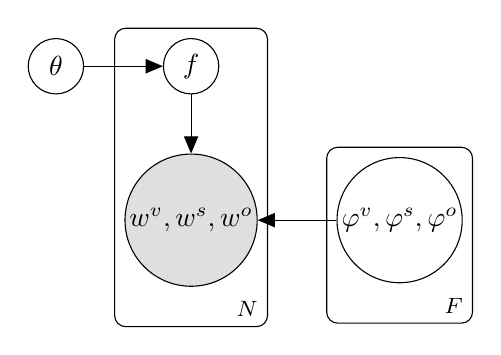
\begin{tikzpicture}
  % Nodes
  \node[obs] (datapoint) {$w^v,w^s,w^o$} ; %
  \node[latent, above=0.75cm of datapoint] (F) {$f$} ; %
  \node[latent, left=of F] (theta) {$\theta$}; %
  \node[latent, right=of datapoint] (phi) {$\varphi^v,\varphi^s,\varphi^o$}; %
  \edge {theta} {F} ; %
  \edge {F} {datapoint}
  \edge {phi} {datapoint} ; %
  \plate {tuples} {(F) (datapoint) } {$N$}; %
  \plate {} {(phi)} {$F$} ; %
\end{tikzpicture}


    \caption{Model 0}
    \label{gen0}

  \end{subfigure}
  \hfill
  \begin{subfigure}[b]{0.45\textwidth}

    \begin{snugshade}
    \scriptsize
    For each frame $f=1..F$:\\
    \hspace*{15pt} For each argument $a\in\{v,s,o\}$:\\
    \hspace*{30pt} Draw a distribution $\phi_f^a\sim Dirichlet(\beta)$\\
    For each document $d=1..D$:\\
    \hspace*{15pt} Draw a distribution $\theta_d \sim Dirichlet(\alpha)$\\
    \hspace*{30pt} For each $i = 1..N^d$:\\
    \hspace*{30pt} Draw a frame $f \sim \theta^d$.\\
    \hspace*{30pt} Draw a verb $v \sim \phi_f^v$\\
    \hspace*{30pt} Draw a subject $s \sim \phi_f^s$\\
    \hspace*{30pt} Draw an object $o \sim \phi_f^o$
    \end{snugshade}

    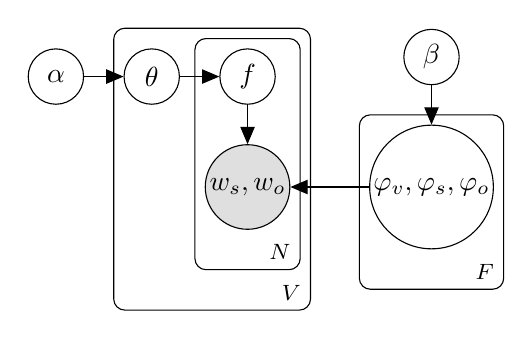
\begin{tikzpicture}[]
    \node[obs]                   (w)     {$w_s,w_o$}; %
    \node[latent, above=0.5cm of w]     (f)     {$f$};
    \node[latent, left=0.5cm of f]     (theta) {$\theta$};
    \node[latent, left=0.5cm of theta] (alpha) {$\alpha$};
    \node[latent, right=of w]    (phi)   {$\varphi_v,\varphi_s,\varphi_o$};
    \node[latent, above=0.5cm of phi] (beta) {$\beta$};
    \edge {alpha} {theta};
    \edge {theta} {f};
    \edge {f} {w};
    \edge {phi} {w};
    \edge {beta} {phi};
    \plate {frames} {(phi)} {$F$};
    \plate {datapoints} {(f) (w)} {$N$};
    \plate {verbs} {(f) (w) (datapoints) (theta)} {$V$};
\end{tikzpicture}


    \caption{Model 1}
    \label{gen1}

  \end{subfigure}

  \caption{Generative Stories}

\end{figure}



\subsection{Model 0}

This approach models each VSO independently, without considering any further context.
Word distributions are completely independent between arguments and across frames.
Tuples are clustered according to which frame's three distributions best fit the 
three arguments; that is,

\[
f_{v,s,o} = \argmax_f P(v|\phi_f^v) \times P(s|\phi_f^s) \times P(o|\phi_f^o)
\]

Model 0 is based on the approach originally proposed in \citet{rooth1999}, which 
considers noun-verb pairs. Following \citet{oconnor2013}, we expand the model
to use the limited syntax of VSOs.

The generative story (figure \ref{gen0}) gives us the following joint probability:
\begin{align*}
P(\mathbf{f},\mathbf{w}|\phi,\theta) 
  =& P(\mathbf{f}|\theta)P(\mathbf{w}|\phi)\\
  =& \prod_{i=1}^{N}\big[\theta(f_i) \prod_a^{\{v,s,o\}}\phi_{f_i}^a(w_i^a)\big]
\end{align*}

Therefore, the incomplete log-likelihood (i.e., where the sequence of frames
is hidden) that we want to maximize is as follows:
\[
L(\theta,\phi) = \sum_{i=1}^N\big[\log \sum_{f_i=1}^F\theta(f_i)\prod_{a}^{\{v,s,o\}}\phi_{f_i}^a(w^a_i)\big]
\]

Expectation maximization can be used to maximize this likelihood.
First we use the current estimates for $\theta$ and $\phi$ to infer a 
distribution over possible choices of frame. This is the E-step. 

\begin{align}
\mu_i(f) =& P(f_i=f, w_i|\phi,\theta)\nonumber\\
=& \frac{\theta(f)\prod_a^{\{v,s,o\}}\phi_f^a(w^a_i)}
                {\sum_{f'=1}^F\theta(f)\prod_a^{\{v,s,o\}}\phi_f^a(w^a_i)}\label{E}
\end{align}

Then in the M-step, we find $\theta$ and $\phi$ that maximize the expectation of
the complete likelihood. In particular, we want to maximize

\begin{align*}
E_\mu\big[\sum_{i=1}^N\log P(w_i,f_i|\theta,\phi)
=& \sum_{i=1}^N\sum_{f=1}^F\mu_i(f)\log\Big[\theta(f)\prod_a^{\{v,s,o\}}\phi_f^a(w_i^a)\Big]\\
=& \sum_{i=1}^N\sum_{f=1}^F\mu_i(f)\log\theta(f)
+ \sum_a^{\{v,s,o\}} \sum_{i=1}^N\sum_{f=1}^F\mu_i(f)\log \phi_f^a(w_i^a)
\end{align*}

Thus the problem is reduced to maximizing each of the terms in the sum above. Fortunately
these have closed for solutions using Lagrangian multipliers.


\begin{align}
\argmax_{\theta(f)}\sum_{i=1}^N\sum_{f=1}^F\mu_i(f)\log\theta(f)
= \frac{\sum_{i=1}^N\mu_i(f)}{\sum_{f'}^F\sum_{i=1}^N\mu_i(f)}
\end{align}

and

\begin{align}
\argmax_{\phi^a(w)}\sum_{i=1}^N\sum_{f=1}^F\mu_i(f)\log \phi_f^a(w_i,a)
= \frac{\sum_{i=1}^N \mu_i(f)\,c(w^a)}{\sum_{w'=1}^{V^a}\sum_{i=1}^N \mu_i(f)\,c(w',a)}
\end{align}

Where $c(w,a)$ indicates the number of times word $w$ is observed as argument $a$.

\subsection{Model 1}

It is in the nature of documents that they have some degree of internal semantic
coherence. Put more plainly, a document is usually \emph{about} something. We
know from topic modeling that LDA with Gibbs sampling can be very successful at
classifying documents according to some semantic features \citep{blei2003}.
Model 1 leverages this fact by making the assumption that a given document is 
likely to have a sparse distribution of frames. As in LDA, the document-level
sparsity is enforced by a Dirichlet prior on frame distributions (see figure
\ref{gen1} for details). This assumption breaks the independence between tuples 
that is maintained by Model 0 is dropped in Model 1.

The independence assumptions in the generative story for model 1 give us the 
following joint distribution:

\begin{align*}
P(\mathbf{w},\mathbf{f}|\theta,\phi,\alpha,\beta)
&=P(\mathbf{w}|\mathbf{f},\phi)\,P(\mathbf{f}|\theta)\,P(\theta|\alpha)\,P(\phi|\beta)
\end{align*}

We can find the marginal distribution of the latent and observed variables by
integrating over the priors:

\begin{align*}
 P(\mathbf{w},\mathbf{f}|\alpha,\beta)
&=\int_\phi\int_\theta P(\mathbf{w},\mathbf{f}|\theta,\phi,\alpha,\beta)\\
&=     \int_\phi P(\mathbf{w}|\mathbf{f},\phi )\,P(\phi|\beta)
\times \int_\theta P(\mathbf{f}|\theta)\,P(\theta|\alpha)\\
\intertext{These integrals are both Dirichlet multinomials:}
&=\frac{DCM_i^{frames}(f_{ij}=f, \mathbf{f}_{-ij})}{DCM_i^{frames}(\mathbf{f}_{-ij})}\times
\prod_a^{\{v,s,o\}}\frac{DCM_i^{vocab^a}(f_{ij}=f, \mathbf{f}_{-ij})}{DCM_i^{vocab^a}(\mathbf{f}_{-ij})}
\end{align*}

We prefer not to consider the subject and object vocabularies independently 
(i.e., $V^s = V^o$). This is more in line with the theory of semantic frames 
since in principle, a noun playing a particular semantic role may appear in either 
syntactic position.

Dropping terms not dependent on counts, we can calculate the proportional
probability required for Gibbs sampling as follows:

\begin{align}
P(f_{ij} = f|\mathbf{f}_{-ij},\mathbf{w}, \alpha,\beta)
&=\frac{\alpha + \tilde c(d_i,f)}{F\,\alpha + \tilde c(d_i)}
\times \prod_a^{\{v,s,o\}}\frac{\beta+\tilde c(f,w_{ij}^a)}{V^a\beta+\tilde c(f)}
\end{align}

Where $\tilde c (d_i, f)$ is the number of VSO's in document $d_i$ assigned to frame $f$;
$\tilde c(d_i)$ is the number of VSO's in document $i$;
$\tilde c(f,w_{ij}^a)$ is the number of VSOs containing $w_{ij}^a$ as argument $a$ that are
assigned to frame $f$; and
$\tilde c(f)$ is the number of VSOs assigned to frame $f$.
Note that $\tilde c$ indicates a count that does not consider the contribution of 
$w_{i,j}$.

The data used in this project (see section \ref{data}) doesn't contain any document-level
information. As a result, we adapt model 1 by grouping VSOs with the same verb into ``documents''.
This move leverages the Dirichlet prior $\alpha$ to enforce sparsity of frames 
across verbs, but of course cannot capture the information given by the kind of
document-level semantic sparsity seen in LDA.\footnote{When we use verbs as
documents (i.e, $D = V^v$), since $w_{ij}^v$ is the same for all verbs in document $d_i$ 
(and $d_i$ is the only document with that verb), it follows that the number of VSO's in document 
$d_i$ belonging to frame $f$ is the same as the number of VSO's with $w_{ij}^v$ as their verb assigned to 
frame $f$; that is, $\tilde c(d_i, f) = \tilde c(f, w_{ij}^v)$.}

\section{Dataset - Verbargs}
\label{data}

A syntactic-ngram is a $k$-word rooted subtree of some sentence.
Google syntactic-ngrams is a corpus of ngrams extracted from 3.5 million English language 
books and labled with Penn Treebank part-of-speech tags Stanford-basic dependency 
labels \citep{ngrams2013}.
Each ngram also includes frequency counts by year.

This project uses the verbargs subeset (130M items) of Google syntactic-ngrams.
An ngram in the verbargs dataset consist of a verb and all of its 
immediate arguments.
We considered only the VSO's in this dataset, that is; we pruned verbargs to
those ngrams containing a subject (nsubj) and object (dobj) whose immediate parent
is the ngram's root verb (1.6M items, 96M by count). 
We further trimmed the data to consider only the \%25 most common verbs 
(800K items, 78M by count).



\section{Experiments}
The number of frames in both models must be determined before induction can take place. When choosing for a low number of frames the clusters will be bigger and thus the meaning of a cluster more vague. In contrast, a high number of frames bears the danger of over-fitting the data, i.e. when unrelated verbs occur with the same arguments often they will be clustered and may even make up one cluster, while with a lower number of frames other verbs would be included, diminishing one of the unrelated verbs as noise. Following \citet{rooth1999}, we estimate that the appropriate number of frames to induce is at most a couple hundred. This assumption is based on philosophical arguments of Jerry Fodor, who proposes that there should be a very limited degree of genuine interdefinability between lexical items (here frames), and that the magnitude of the lexicon should therefore be approximately equal to the number of basic concepts \citep{fodor1998}.

To facilitate the evaluation of our results, we split off two uniform random subsets of the data, the test set (\%10), and the cross-verb validation set (\%20). We trained the models on the remaining data (the training set). To train the baseline model (model 0), we ran the expectation maximization algorithm until the total change in the posterior probabilities for words plus the prior for frames was less that $0.01$. The trained model consists of $3\times|Frames|$ distributions: a distribution for each frame, for each argument. Model 1 is implemented using Gibbs sampling. We allowed $1000$ iterations of sampling, ignoring the first $50$ as \emph{burn in} (see \citet{raftery1992} for further discussion). Since we are less na\"ive about mapping syntactic positions to semantic roles, we combine the subject/object distributions, so model 1 gives $2\times|Frames|$ distributions: for each frame, one for verbs and one for nouns.

The $\alpha$ and $\beta$ hyperparameters in model 1 are known  to be hard to determine \citep{oconnor2013}, and therefore need to be experimentally optimized for our specific problem. We used an expensive, but easy to implement grid search to determine the best values for $\alpha$ and $\beta$. The grid search builds, for each posible parameter set, a model which is evaluated on the cross validation set. The highest scoring model is tested with the test set. We ran grid search for model 0 on $50$ - $200$ frames, with steps of $50$, and $\alpha$ of $0.1, 0.5, 1, 1.5$, and $2$. The grid search for Model 1 was the the same, additionally testing $\beta$ across the same values as $\alpha$
\section{Results}
\label{results}

\subsection{Frame Coherency}
Verb clusters are based on the arguments with which they occurring in the data. So to test how well the models perform on clustering, the probability that the model generates a triple from the testset, should be greater than this triple with a random verb in place of the real one. This metric is the same as the one used by \citeauthor{rooth1999}. More formally: for a datapoint $(v,s,o)$ and a tuple $(v^r,s,o)$ where $v^r$ is a random chosen verb: $P(v\mid s,o) \geq P(v^r\mid s,o)$.
The results are percentages of data points which satisfy this condition. Note though that if the random verb-triple is assigned the same frame as its `parent' real triple, this metric loses its meaning, but since the number of frames is high this probability is low. Furthermore, one can assume that the occurrences of same frame assignment cancel each other out, i.e. the random triple has higher probability than the real one as many times as vice versa.

\subsection{Frame Correctness}
% I (Eli) can expond here on the relation/contrast/etc.
%   between what we're doing and FrameNet;
%   I think O'Connor brings up some technical and/or methodological points
%   about ways we can vs. can't use the FN data for evaluating
%   induction and such, I'll look it over again.

%\subsection{Relation to FrameNet}

The FrameNet project is a manually compiled and annotated database for frame semantics. It tracks frames, the cast of elements that play specified roles within each frame, individual word-senses (``lexical units'' in FrameNet-speak) that instantiate those elements, certain relationships between frames, examples, etc. 

We want to compare our induced frames to FrameNet's manually annotated (i.e. correct) frames.
In our case, we restrict our attention to sets of verbs.
The idea is that if the verb groups identified by our model are actually groups that belong together in a frame, there should be a FrameNet frame that includes these verbs as well. Inclusion of a word in FrameNet frame for us simply means that the word is a lexical unit for that frame; since lexical units are tagged with parts of speech, extracting verbsets for each frame is simple.
%Following the example of \citeauthor{oconnor2013}, we do not consider FrameNet frames with a very small number of verbs

We can thus compute a rough ``correctness'' measure for our models' induced frames by comparing their verbsets with the verbsets extracted from FrameNet, using the Dice coefficient as a similarity measure. For verbsets $M$ and $F$ of some model-induced frame and some FrameNet frame, respectively, their Dice similarity is \[\frac{2|M\cap F|}{|M|+|F|}\]
% Dice has certain properties that work well in this situation.
For each FrameNet frame, we can find the frame given by our model that is most Dice-similar.
Ideally, we want each FrameNet frame to have a high-scoring match among the frames of our model.
%and also for these matches not to be identical

One issue with implementing this measure is that our models return probability distributions, not verbsets. Specifically, for each induced frame, we have a distribution over all verbs from our dataset. To compare these frames with those from FrameNet using Dice, however, we need to turn these distributions into discrete sets, and there is not a clear method to do this.
%(It is important to keep in mind that the collection of verbsets is not a partition on the set of all verbs appearing in the data, since each verb can appear in more than one frame (indeed, some of the most interesting test cases for automated frame inductors involve such multi-frame verbs).)
We can take the most probable $n$ (say, five) verbs for each frame, but this will likely run into problems in the case of both high-population and low-population frames. Alternatively, we can take verbs within a given frame with a probability greater than some threshold value $p$ (say, $0.02$), which may perform better in certain cases but risks returning empty verbsets for frames with distributions that are particularly spread out.




There are some substantial methodological issues with this approach even if it does function as a general evaluation method. 

Although many frames are events and thus commonly feature verbs as core elements, FrameNet is not verb-centric by design. Some frames do not encompass events and include no verbs at all.
FrameNet also imposes inheritance relations between frames. Our model could potentially identify verbsets that have these relations, though it has no way of recognizing it has done so.
In short, to use FrameNet's data, we end up discarding most of the information in the annotations and using only a fraction of the frames and lexical units. Arguably this is not so much of an issue so long as the extracted verbsets are still useful in evaluating our own model, even if the FrameNet data is being used in an idiosyncratic way.

Perhaps a more important point, though, is that completeness is not a primary goal for FrameNet. Not every English word is included as a lexical unit, and not all words that are included are fully annotated with all their senses as lexical units in appropriate frames.
In practice this means that if our model induces a certain verbset that does constitute a coherent semantic frame, but some of the verbs in the set do not show up in the FrameNet data for whatever reason, that frame's Dice score will suffer.
% 




On a more abstract level, to what extent do lower similarity scores with FrameNet necessarily mean our model has identified frames that are semantically ``incorrect'' as opposed to frames which are in a sense orthogonal?
% Does this make sense? Maybe this should go in "Discussion"..?





%Frame correctness: for the top 25 most probable verbs per frame $TV$ and framenet classes of verbs $FN$: \[\frac{2|TV\cap FN|}{|TV|+|FN|}\]


\subsection{Model 0}

\subsection{Model 1}


\section{Discussion}


\section{Future Work}
One big weakness of this project over the results of \citet{oconnor2013} is that 
we could not used document-level context to infer semantic information.
A possible direction of future research is to create models that take better 
advantage of the syntax-level context provided by syntactic ngrams. 
One easy way to do this would be to modify model 1 so that the argument 
vocabulary ranges over subject/object pairs instead of individual nouns.
or object.
More advanced models might take better advantage of the various kinds of arguments
in the verbargs dataset and their relation to one another.
For example, you could be glean some semantic information about the relationship between
verbs and prepositional objects by looking at the preposition that mediates them: 
That you ''swim \emph{in} a lake'' versus ``ice skate \emph{on} a lake'' 
indicates that the relationship between swimming and lakes is different from the one between
ice skating and lakes.

\section{Conclusion}


\bibliography{refs.bib}

\end{document}
